\documentclass[uplatex,dvipdfmx,a4paper,10pt,twocolumn]{bxjsarticle}

\usepackage[dvipdfmx]{graphicx}
\usepackage[dvipdfmx,colorlinks=true,allcolors=blue!55!black]{hyperref}
\usepackage{amsmath,amssymb,bm,booktabs,array,multirow}
\usepackage{geometry}
\usepackage{xcolor}
\usepackage{url}
\usepackage{enumitem}

\geometry{top=18mm,bottom=20mm,left=17mm,right=17mm}
\setlength{\columnsep}{6mm}
\setlength{\textfloatsep}{8pt plus 2pt minus 2pt}
\setlength{\floatsep}{7pt plus 2pt minus 2pt}
\setlength{\intextsep}{7pt plus 2pt minus 2pt}
\setlist[itemize]{leftmargin=1.5em,itemsep=1pt,topsep=2pt}
\graphicspath{{figures/}}

\newcommand{\R}{\mathbb{R}}
\newcommand{\RSN}{RSN}
\newcommand{\knn}{KNN}
\newcommand{\good}{\mathop{\uparrow}}
\newcommand{\low}{\mathop{\downarrow}}

\title{\bfseries \RSN：クラス条件付きロバスト標準化近傍距離による\\
野生動物画像の超近接分布外検知}
\author{d-hacks B3.0 omote \quad / \quad 親:zackeyさん}
\date{}

\begin{document}
\maketitle

\begin{abstract}
同一分類群内の超近接 OOD 検知では，既知種と未知種の特徴が重なりやすい．本稿では，クラス別の次元標準偏差による正規化と Huber 集約を組み合わせた \RSN を提案する．ネコ科8種・105,554枚，$m=2$--7の全1,476 foldで21手法を比較し，\RSN は $m=2$--4の全3指標で首位，6サイズ平均順位でも AUROC 2.50，FPR95 1.33，AUPR-OUT 2.17で首位となった．一方，$m=5$--7では OpenMax と RMD が一部指標で上回り，ID クラス数による順位転換も確認した．
\end{abstract}

\section{はじめに}

深層画像分類器は，学習時に観測していない入力に対しても高い確信度を返すことがある~\cite{hendrycks2017baseline}．この問題を扱う OOD 検知は，分類結果を生態調査や保全判断へ接続する野生動物認識で特に重要である~\cite{norouzzadeh2018automatically,tuia2022perspectives}．誤った既知種判定は，個体数推定，希少種発見，外来種監視の下流処理へそのまま伝播するためである．

従来の評価では，ID と OOD が視覚的に大きく異なる設定も多い．一方，実際の種同定では，未知種が既知種と同じ科に属し，体型，毛皮模様，姿勢，背景が強く類似する．本研究では，このように同一ドメイン・同一分類群の種のみで ID/OOD を構成する設定を\textbf{超近接 OOD（Ultra-Near-OOD）}と呼ぶ．対象は cheetah，jaguar，leopard，lion，ocelot，puma，serval，tiger の8種であり，jaguar，leopard，ocelot のロゼット模様など，未知種を既知種へ近づける視覚要因を含む．

凍結特徴に対する \knn は，分類 head に依存せず，局所密度を利用できる強い基準である~\cite{sun2022knn}．しかし通常の \knn は，すべてのクラスを同一の等方的距離で測る．姿勢や背景の変動が大きいクラスと均質なクラスでは，各特徴次元の自然な変動幅が異なるため，生の距離はクラス間で同じ意味を持たない．また低分散な一方向だけの偶発的なずれが，標準化距離全体を過度に押し上げる場合がある．

\newpage
そこで本稿では \RSN を提案する．主な貢献を以下に示す．
\begin{itemize}
  \item クラス条件付き次元別標準化と Huber 集約を組み合わせた，学習不要・較正不要の近傍 OOD score を定義する．
  \item 105,554枚のクリーニング後データで，全 ID 組合せ $\times$ 3 seed $\times$ 2 DINOv2 backbone，計1,476 foldについて21手法を比較し，ID クラス数に伴う順位転換まで示す．
  \item 全手法を同一 split・特徴・分類 head の下で評価し，fold-level paired 比較，信頼区間，完全性監査を含む再現可能な評価手順を提示する．
\end{itemize}

\section{関連研究}

\subsection{分類 head に基づく OOD 検知}

MSP~\cite{hendrycks2017baseline} は最大 softmax 確率を ID らしさとする．Energy~\cite{liu2020energy}，MaxLogit，Entropy，GEN~\cite{liu2023gen} は，同じ logit から異なる集約を構成する．GradNorm~\cite{huang2021gradnorm} は分類層勾配，OpenMax~\cite{bendale2016openmax} は EVT による未知クラス確率を用いる．これらは軽量である一方，ID クラス間識別のための head が超近接 OOD に高い logit を与えると，score 全体が影響を受ける．本稿では共通の決定論的 ridge 線形 head を用い，head 依存手法間の学習条件を揃える．

\subsection{特徴距離に基づく OOD 検知}

Mahalanobis 法~\cite{lee2018simple} はクラス条件付きガウス分布を仮定し，共有共分散による距離を用いる．RMD~\cite{ren2021simple} はクラス距離から背景分布の距離を差し引き，Mahalanobis++~\cite{muller2025mahalanobispp} は特徴正規化を導入する．ViM~\cite{wang2022vim} は分類 logit と特徴残差を結合する．\knn~\cite{sun2022knn} は分布形の仮定を置かず，正規化特徴の近傍距離を用いる．

\RSN は \knn と同じ近傍探索を基礎とするが，距離をクラスごとの次元別スケールへ適応させる．フル共分散の逆行列を推定せず，$D$ 個の標準偏差だけを推定する点で Mahalanobis 系とも異なる．さらに，標準化後の各座標を二乗和へ直接入れず Huber 化し，単一座標の影響を抑える．

\section{提案手法}

図~\ref{fig:pipeline} に主設定の処理を示す．\textbf{生の DINOv2 特徴，$k=150$，全 ID クラス候補，Huber $\delta=1.345$，較正なし}を用いる．

\begin{figure*}[t]
  \centering
  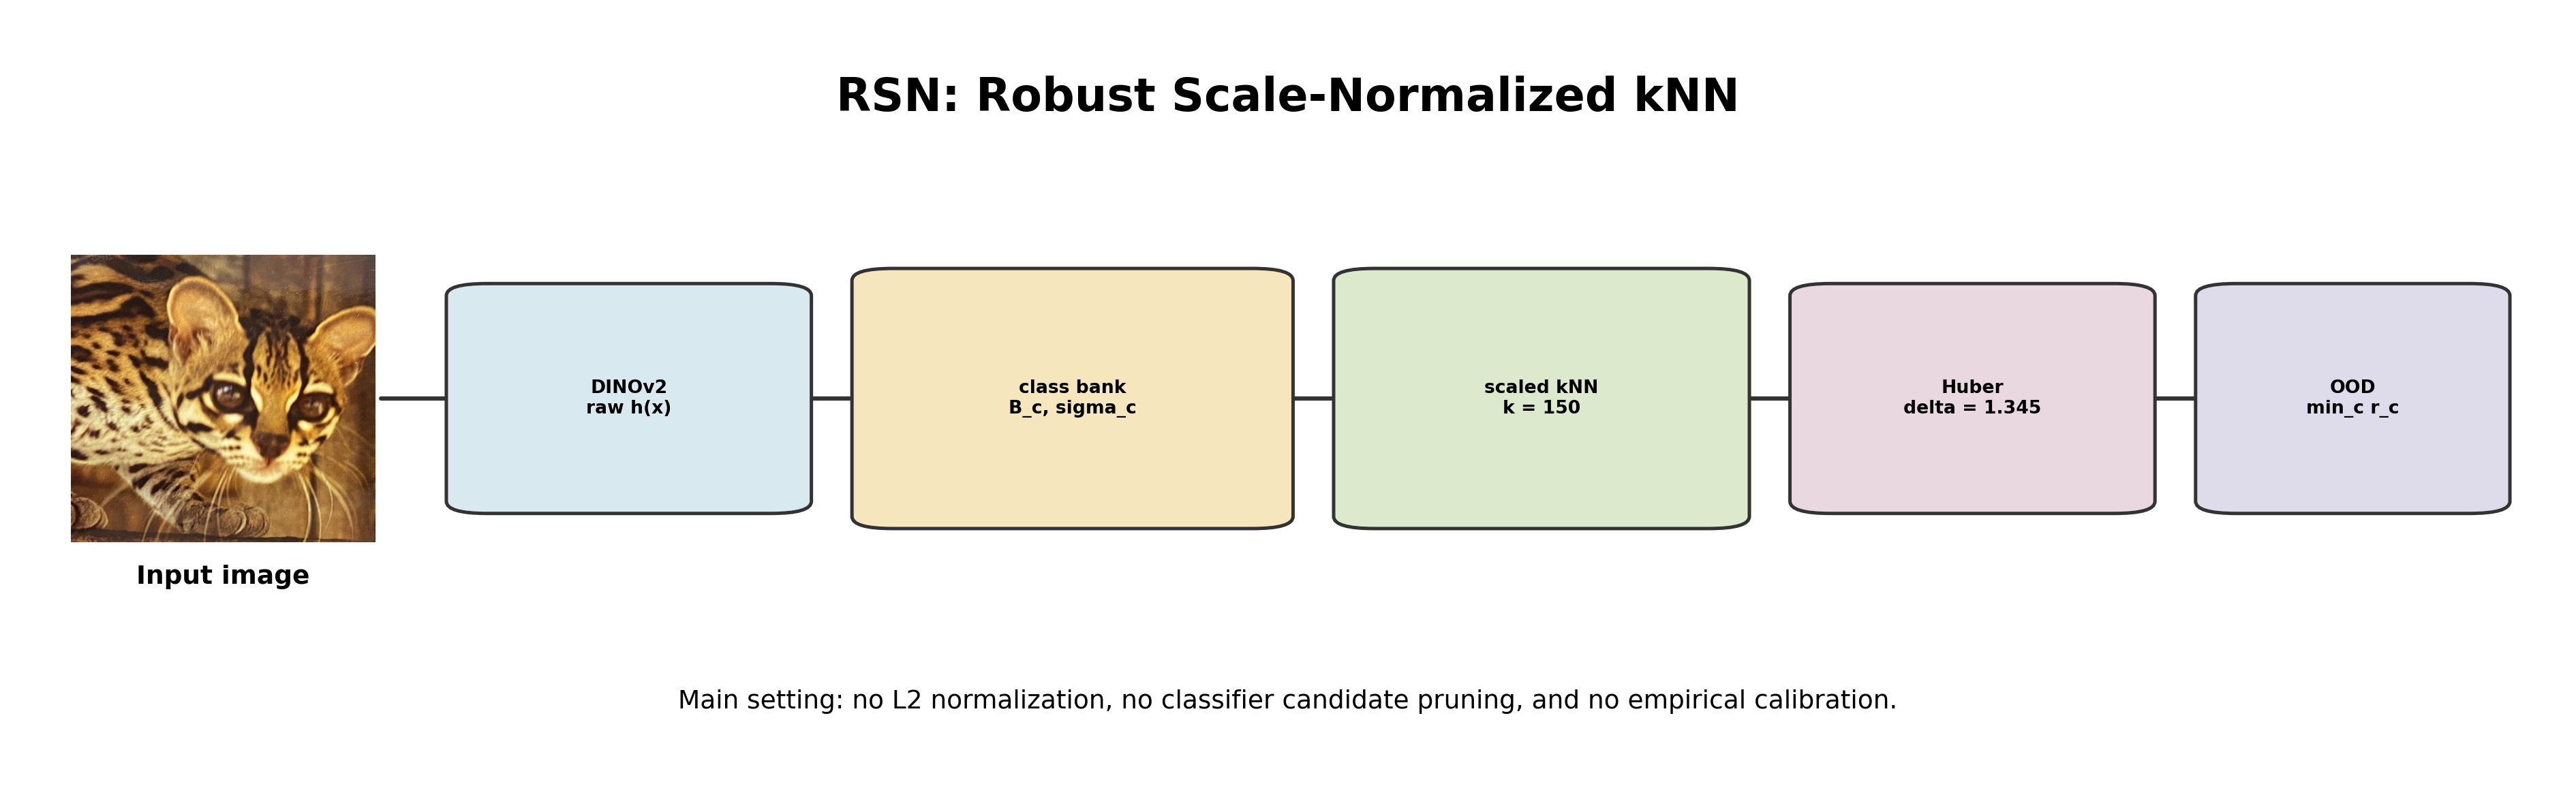
\includegraphics[width=0.98\textwidth]{fig01_rsn_pipeline.png}
  \caption{\RSN の主設定．生の DINOv2 CLS 特徴からクラス別バンクと次元別標準偏差を作り，各クラスで標準化後の150近傍を求める．Huber 集約後，すべての ID クラスに対する最小距離を OOD score とする．$\ell_2$ 正規化，top-$q$ 候補制限，経験分位点較正は用いない．}
  \label{fig:pipeline}
\end{figure*}

\subsection{生特徴とクラス別スケール}

凍結 backbone の CLS 特徴を
\begin{equation}
  h(x)\in\R^D
\end{equation}
とし，主設定では $\ell_2$ 正規化しない．ID クラス $c$ の train 特徴バンクを
\begin{equation}
  \mathcal{B}_c=\{h_i\mid y_i=c\}
\end{equation}
とする．各次元 $d$ の標準偏差は
\begin{equation}
  \sigma_{c,d}=\max\!\left(\mathrm{std}\{h_i^{(d)}:h_i\in\mathcal{B}_c\},\tau\right),
  \quad \tau=10^{-3}
  \label{eq:sigma}
\end{equation}
で推定する．対角スケールだけを用いるため，推定パラメータ数はクラスあたり $D$ であり，共分散の $O(D^2)$ パラメータや逆行列を必要としない．

\subsection{標準化近傍と Huber 集約}

クラス $c$ に対し，問い合わせとバンクをそれぞれ $\bm{h}/\bm{\sigma}_c$ で標準化し，Euclidean 距離が小さい $k=150$ 点の添字集合を $N_k^c(x)$ とする．近傍 $i$ の次元別残差は
\begin{equation}
  t_{c,i}^{(d)}(x)=\frac{h^{(d)}(x)-h_i^{(d)}}{\sigma_{c,d}}.
\end{equation}
標準化により低分散次元のずれを検出しやすくなる一方，単一次元の偶発的な外れ値も増幅される．そこで実装と一致する Huber 型関数
\begin{equation}
\rho_\delta(t)=
\begin{cases}
t^2,& |t|\le\delta,\\
2\delta|t|-\delta^2,& |t|>\delta
\end{cases},\qquad \delta=1.345
\label{eq:huber}
\end{equation}
を用いる~\cite{huber1964robust}．クラス距離は
\begin{equation}
  r_c(x)=\frac{1}{k}\sum_{i\in N_k^c(x)}\sum_{d=1}^{D}
  \rho_\delta\!\left(t_{c,i}^{(d)}(x)\right)
  \label{eq:classdistance}
\end{equation}
である．$\rho$ は小さい残差を二乗で保持し，大きい残差を線形へ切り替える．

\subsection{OOD score}

最終 score は全 ID クラスに対する最小値
\begin{equation}
  o_{\RSN}(x)=\min_{c\in\mathcal{C}_{\mathrm{ID}}}r_c(x)
  \label{eq:score}
\end{equation}
とし，大きいほど OOD とする．分類 head の top-$q$ で候補を削らないため，head の誤分類で正しい近傍クラスが除外されない．全バンクを走査する主項は通常の brute-force \knn と同じ $O(ND)$ で，その後の Huber 集約は $O(CkD)$ である．実験では GPU 上でクラス・問い合わせを batch 化する．

\subsection{較正を用いない理由}

クラス特徴が $h_c=\mu_c+\sigma_c\odot u$，かつ潜在分布 $u$ がクラス間で共有されるなら，式~\eqref{eq:sigma}の標準化後は $r_c$ の ID 分布が共通分布 $F$ に近づく．このとき経験分位点 $q_c(x)=1-F(r_c(x))$ を追加しても，
\begin{equation}
  \arg\max_c q_c(x)=\arg\min_c r_c(x)
\end{equation}
であり，score の単調変換にすぎない．有限 validation からクラス別 $\hat F_c$ を再推定すると，DKW 不等式~\cite{dkw1956}
\begin{equation}
  \Pr\!\left(\sup_r|\hat F_c(r)-F_c(r)|>\epsilon\right)
  \le 2e^{-2n_c\epsilon^2}
\end{equation}
の推定誤差がクラスごとに加わる．したがって，対角標準化でスケール差が十分小さくなった場合，較正は情報利得より順位ノイズを増やしうる．実験ではこの仮説を4条件 ablation と分布形状の直接比較で検証する．

\section{実験設定}

\subsection{CAT データセット}

ウェブ収集画像に対し，完全重複・近重複のグループ化と，明白な別内容，足跡のみ，地図・画面等の除外を行った．最終枚数は表~\ref{tab:counts}の105,554枚である．自動クリーニング後も誤ラベルが完全にゼロとは仮定しないが，実験に用いた manifest の実測枚数は期待値と全クラスで一致した．重複群が train/validation/test を跨がないよう，クラス内で4:1:1に分割した．

\begin{table}[t]
\centering
\caption{クリーニング後 CAT データセット．}
\label{tab:counts}
\begin{tabular}{lr@{\hspace{7mm}}lr}
\toprule
種 & 枚数 & 種 & 枚数\\
\midrule
cheetah & 11,349 & ocelot & 12,342\\
jaguar  & 10,452 & puma   & 18,763\\
leopard & 10,984 & serval &  9,149\\
lion    & 15,845 & tiger  & 16,670\\
\midrule
\multicolumn{3}{r}{合計} & 105,554\\
\bottomrule
\end{tabular}
\end{table}

8種から $m=2,3,4,5,6,7$ 種を ID として選び，残りを OOD とする全組合せを評価した．seed は0,1,2，backbone は DINOv2 ViT-B/14 と ViT-L/14~\cite{oquab2024dinov2}である．各 $m$ の fold 数は $\binom{8}{m}\times3\text{ seed}\times2\text{ backbone}$ で決まり，内訳を表~\ref{tab:folds}に示す．OOD train/validation は用いず，protocol は fair のみとした．

\begin{table}[t]
\centering
\small
\caption{ID クラス数ごとの評価 fold 数．}
\label{tab:folds}
\begin{tabular}{crrrr}
\toprule
$m$ & ID 組合せ数 & seed & backbone & fold数\\
\midrule
2 & $\binom{8}{2}=28$ & 3 & 2 & 168\\
3 & $\binom{8}{3}=56$ & 3 & 2 & 336\\
4 & $\binom{8}{4}=70$ & 3 & 2 & 420\\
5 & $\binom{8}{5}=56$ & 3 & 2 & 336\\
6 & $\binom{8}{6}=28$ & 3 & 2 & 168\\
7 & $\binom{8}{7}=8$  & 3 & 2 & 48\\
\midrule
合計 & 246 & -- & -- & 1,476\\
\bottomrule
\end{tabular}
\end{table}

\subsection{比較手法と実装条件}

主比較は正規化特徴を用いる \knn（$k=50$）である．さらに MSP，Entropy，Energy，MaxLogit，GEN，GradNorm，KL-Matching，Mahalanobis，Mahalanobis++，RMD，ViM，ReAct，ASH-P/B/S，DICE，SCALE，NCI，OpenMax を含む20ベースラインを，$m=2$--7の全 foldで評価した．\RSN を加えた主ランキングは21手法である．分類器依存手法には，ID train の生 DINOv2 特徴から学習した共通の閉形式 ridge 線形 probe（$\lambda=10^{-3}$，bias は非正則化）を用い，early stopping は行わない．

特徴統計，共分散，近傍 bank，分類 head は各 fold の ID train のみから推定する．OOD train/validation は使用せず，手法固有のハイパーパラメータも全 foldで固定した．入力画像への勾配や別 encoder を必要とする方法は比較範囲に含めない．主設定，20ベースライン，1感度設定の計22設定について32,472 jobsを実行し，期待ジョブとの照合，raw score fingerprint，欠測・重複・非有限値を fold単位で検査した．

\subsection{評価指標}

OOD を positive とし，AUROC$\good$，FPR95$\low$，AUPR-OUT$\good$ を報告する．表の平均は fold-level 指標の算術平均である．手法比較では backbone，seed，ID set を揃えた paired 差を用い，$t$ 分布近似の95\%信頼区間と good rate（\RSN が改善した fold 比率）を求めた．

\section{結果}

\subsection{ID クラス数 $m=2$--7 の主結果}

表~\ref{tab:idsize}および図~\ref{fig:idsize}に，$m=2,3,4,5,6,7$ の全結果を示す．これは本研究の主比較であり，合計1,476 foldを含む．\RSN はすべての $m$ で，\knn より AUROC と AUPR-OUT が高く，FPR95 が低い．ID クラスが増えるほど OOD 側の残りクラスが減り，難しいロゼット種が評価に占める組合せ効果も強くなるため，絶対性能は低下するが，\knn に対する優位は維持される．

\begin{table*}[t]
\centering
\scriptsize
\setlength{\tabcolsep}{5.0pt}
\caption{ID クラス数 $m=2$--7 の主比較（2 backbone pooled）．A=AUROC，F=FPR95，P=AUPR-OUT．太字は各 $m$ の最良値．}
\label{tab:idsize}
\begin{tabular}{crrrrrrr}
\toprule
$m$ & $n$ & \multicolumn{3}{c}{\RSN} & \multicolumn{3}{c}{\knn}\\
 & & A & F & P & A & F & P\\
\midrule
2 & 168 & \textbf{.9169} & \textbf{.4307} & \textbf{.9590} & .9126 & .4626 & .9560\\
3 & 336 & \textbf{.8965} & \textbf{.5005} & \textbf{.9125} & .8910 & .5373 & .9053\\
4 & 420 & \textbf{.8788} & \textbf{.5528} & \textbf{.8431} & .8729 & .5951 & .8311\\
5 & 336 & \textbf{.8624} & \textbf{.5952} & \textbf{.7418} & .8565 & .6401 & .7255\\
6 & 168 & \textbf{.8454} & \textbf{.6336} & \textbf{.5953} & .8397 & .6835 & .5775\\
7 &  48 & \textbf{.8224} & \textbf{.6857} & \textbf{.3881} & .8171 & .7355 & .3729\\
\bottomrule
\end{tabular}
\end{table*}

\begin{figure*}[t]
  \centering
  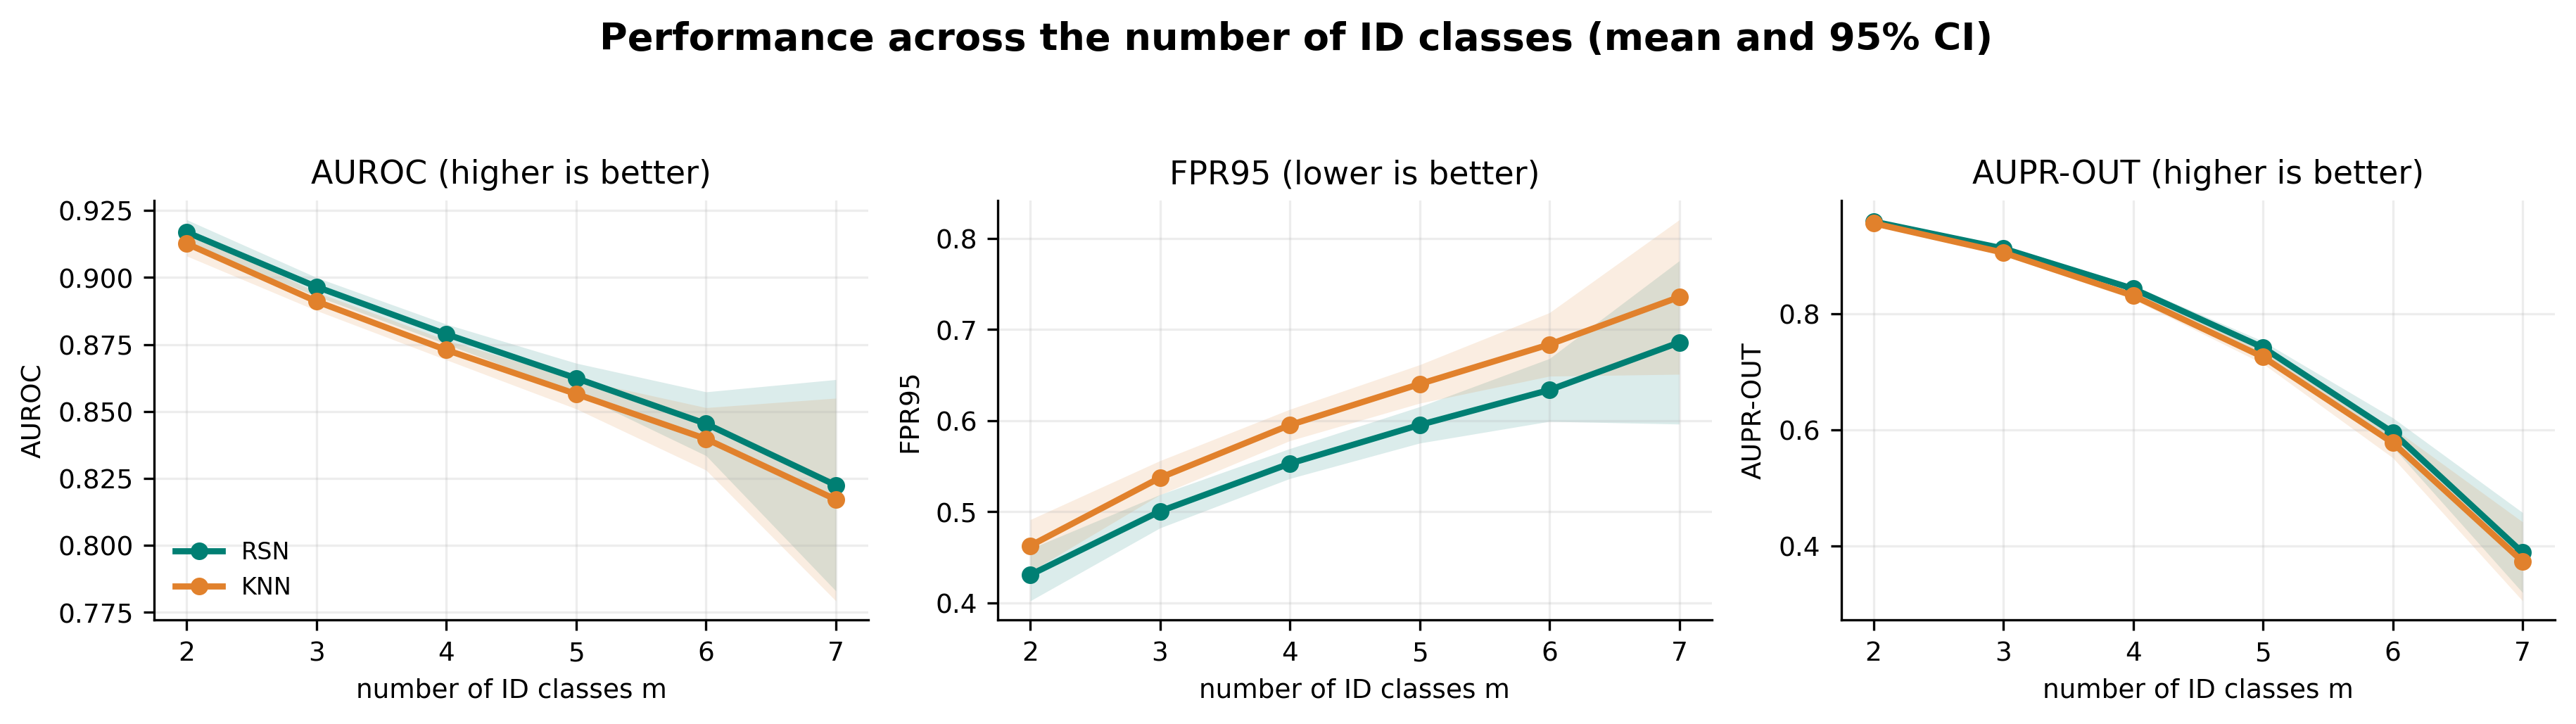
\includegraphics[width=0.98\textwidth]{fig02_idsize_trend.png}
  \caption{ID クラス数 $m=2$--7 に対する pooled AUROC，FPR95，AUPR-OUT．帯は fold間95\%信頼区間．\RSN は全18条件（6 sizes $\times$ 3 metrics）で \knn を上回る．}
  \label{fig:idsize}
\end{figure*}

$m=2$ の ViT-B/14では \RSN/\knn の AUROC は0.9107/0.9055，ViT-L/14では0.9230/0.9197であり，モデル規模によらず順位が一致した．全 $m$ の backbone 別でも同じ順位である．

\subsection{全21手法の横断比較（$m=2$--7）}

表~\ref{tab:fullsweep}に各 $m$ の指標別首位と \RSN の順位を示す．\RSN は $m=2,3,4$ の全3指標で首位である．$m=5$ 以降は AUROC で OpenMax，AUPR-OUT で RMD が首位となり，$m=6,7$ の FPR95も RMD が最小となる．一方，6サイズを等重みで平均した \RSN の順位は AUROC 2.50，FPR95 1.33，AUPR-OUT 2.17であり，3指標すべてで21手法中最良である．

\begin{table*}[t]
\centering
\scriptsize
\setlength{\tabcolsep}{3.1pt}
\caption{全手法比較の指標別首位と \RSN の順位（2 backbone pooled）．括弧内は \RSN の順位．}
\label{tab:fullsweep}
\begin{tabular}{crlrrlrrlrr}
\toprule
$m$ & $n$ & \multicolumn{3}{c}{AUROC} & \multicolumn{3}{c}{FPR95} & \multicolumn{3}{c}{AUPR-OUT}\\
 & & 首位 & 値 & RSN順位 & 首位 & 値 & RSN順位 & 首位 & 値 & RSN順位\\
\midrule
2 & 168 & \RSN & .9169 & (1) & \RSN & .4307 & (1) & \RSN & .9590 & (1)\\
3 & 336 & \RSN & .8965 & (1) & \RSN & .5005 & (1) & \RSN & .9125 & (1)\\
4 & 420 & \RSN & .8788 & (1) & \RSN & .5528 & (1) & \RSN & .8431 & (1)\\
5 & 336 & OpenMax & .8658 & (2) & \RSN & .5952 & (1) & RMD & .7562 & (3)\\
6 & 168 & OpenMax & .8534 & (4) & RMD & .6245 & (2) & RMD & .6339 & (3)\\
7 &  48 & OpenMax & .8343 & (6) & RMD & .6439 & (2) & RMD & .4422 & (4)\\
\bottomrule
\end{tabular}
\end{table*}

OpenMax の AUROC は $m=5,6,7$ で平均上 \RSN を上回るが，paired 差（\RSN$-$OpenMax）の95\% CIは順に $[-.0088,.0020]$，$[-.0163,.0002]$，$[-.0331,.0095]$ で0を跨ぐ．対して RMD の AUPR-OUT は $m=5,6,7$ で有意に高く，差（\RSN$-$RMD）は $-.0144$，$-.0386$，$-.0542$，各95\% CI上端も負である．したがって，\RSN の強みは少数IDクラスでの総合首位と，全サイズでの安定した低FPR95であり，高 $m$ の AUPR-OUTでは RMD に明確な優位がある．

\subsection{主設定の選択と ablation}

表~\ref{tab:ablation}に，較正・Huber の2$\times$2 ablationと，$\ell_2$ 正規化・$k=10$・top-3設定との比較を示す．生特徴・$k=150$・全クラスを用いる \RSN が最良である．$\ell_2$/10/top-3との差には，特徴ノルム情報の除去，近傍数の減少，head による候補制限の3要因が含まれるため，単一要因の効果とは解釈しない．

\begin{table}[t]
\centering
\scriptsize
\caption{設定・較正・Huber ablation（$m=2$, $n=168$）．}
\label{tab:ablation}
\begin{tabular}{lrrr}
\toprule
設定 & AUROC & FPR95 & AUPR\\
\midrule
\textbf{\RSN (raw, $k=150$, all)} & \textbf{.9169} & \textbf{.4307} & \textbf{.9590}\\
\RSN$-$Huber & .9164 & .4362 & .9583\\
\RSN$+$calib$+$Huber & .9126 & .4706 & .9563\\
\RSN$+$calib & .9119 & .4776 & .9555\\
$\ell_2$, $k=10$, top-3 & .9086 & .4522 & .9561\\
\knn & .9126 & .4626 & .9560\\
\bottomrule
\end{tabular}
\end{table}

全1,476 foldで \RSN と \RSN$-$Huber を paired 比較すると，AUROC $+0.000363$（95\% CI $[0.000344,0.000382]$），FPR95改善 $0.005766$（$[0.005448,0.006085]$），AUPR $+0.001773$（$[0.001702,0.001844]$）であった．効果量は小さいが方向は安定し，good rate はそれぞれ87.7\%，88.1\%，97.7\%である．

\subsection{全fold paired 比較}

表~\ref{tab:paired}は全 $m$ を併合した \knn との paired 結果である．FPR95については「\knn の FPR95 $-$ \RSN の FPR95」を改善量として正値で表す．\RSN は平均 AUROCを$+0.00556$，AUPR-OUTを$+0.01163$改善し，FPR95を0.04156低減した．

\begin{table}[t]
\centering
\scriptsize
\caption{全fold paired 比較（$n=1,476$）．}
\label{tab:paired}
\begin{tabular}{lrrr}
\toprule
指標 & 平均改善 & 95\% CI & good\\
\midrule
AUROC & .00556 & [.00494,.00618] & 70.0\%\\
FPR95 & .04156 & [.03817,.04495] & 72.2\%\\
AUPR & .01163 & [.01056,.01270] & 71.5\%\\
\bottomrule
\end{tabular}
\end{table}

事前に定めた2比較（\knn および \RSN$-$Huber）を6 id sizeで検定する12比較に Bonferroni 補正（$\alpha/12$）を適用しても，$m=2$--6の \RSN vs. \knn は3指標で有意であった．$m=7$ は $n=48$ と小さく，\knn 比の区間が0を跨ぐため，このサイズ単独の有意性は主張しない．

\subsection{未知種別の難しさ}

表~\ref{tab:perood}に $m=2$ の per-OOD-class 結果を示す．tiger と lion は比較的分離しやすい一方，jaguar，leopard，ocelot は AUROC 0.840--0.847に留まる．3種はいずれもロゼット模様を持ち，既知側に別の斑紋種が含まれる fold で視覚的近傍へ入りやすい．ocelot の FPR95 0.711は特に高く，平均 AUROCだけでは見えない閾値近傍の誤受理が残る．

\begin{table}[t]
\centering
\scriptsize
\caption{$m=2$ における \RSN の未知種別評価．}
\label{tab:perood}
\begin{tabular}{llrrr}
\toprule
OOD種 & 模様 & AUROC & FPR95 & AUPR\\
\midrule
jaguar  & ロゼット & .8395 & .6262 & .6357\\
leopard & ロゼット & .8465 & .5824 & .6679\\
ocelot  & ロゼット & .8471 & .7112 & .6435\\
puma    & 無地     & .9307 & .4781 & .8490\\
cheetah & 斑点     & .9355 & .4851 & .7810\\
serval  & 斑点     & .9375 & .4190 & .7754\\
lion    & 無地     & .9612 & .2894 & .8883\\
tiger   & 縞       & .9783 & .0703 & .9535\\
\bottomrule
\end{tabular}
\end{table}

\begin{table*}[!t]
\centering
\tiny
\setlength{\tabcolsep}{1.35pt}
\caption{全21手法のIDクラス数別 AUROCと6サイズ平均 AUROC順位 $\bar r_A$．非主設定の感度条件は除く．}
\label{tab:fullranking}
\begin{tabular}{lrrrrrrr@{\hspace{3mm}}lrrrrrrr}
\toprule
手法 & $m{=}2$ & $m{=}3$ & $m{=}4$ & $m{=}5$ & $m{=}6$ & $m{=}7$ & $\bar r_A$ &
手法 & $m{=}2$ & $m{=}3$ & $m{=}4$ & $m{=}5$ & $m{=}6$ & $m{=}7$ & $\bar r_A$\\
\midrule
\RSN & .9169 & .8965 & .8788 & .8624 & .8454 & .8224 & 2.50 & Energy & .8439 & .8660 & .8624 & .8480 & .8286 & .8049 & 10.50\\
OpenMax & .8440 & .8738 & .8741 & .8658 & .8534 & .8343 & 3.17 & SCALE & .8343 & .8579 & .8533 & .8466 & .8246 & .8048 & 11.67\\
\knn & .9126 & .8910 & .8729 & .8565 & .8397 & .8171 & 4.17 & KL-Matching & .7996 & .8335 & .8380 & .8362 & .8328 & .8227 & 12.00\\
MSP & .8440 & .8717 & .8709 & .8607 & .8475 & .8304 & 4.33 & Mahalanobis++ & .8987 & .8693 & .8449 & .8232 & .8016 & .7736 & 12.50\\
MaxLogit & .8440 & .8705 & .8695 & .8591 & .8456 & .8284 & 5.83 & DICE & .8792 & .8430 & .8042 & .7644 & .7219 & .6764 & 15.00\\
Entropy & .8440 & .8686 & .8660 & .8530 & .8353 & .8130 & 7.50 & NCI & .7989 & .8293 & .8328 & .8250 & .8122 & .7934 & 15.17\\
GradNorm & .8430 & .8706 & .8676 & .8525 & .8306 & .8015 & 9.00 & ReAct & .6006 & .6443 & .6746 & .6815 & .6760 & .7464 & 17.83\\
GEN & .8440 & .8679 & .8641 & .8498 & .8304 & .8068 & 9.00 & ASH-S & .4879 & .5022 & .5252 & .5436 & .5347 & .5498 & 19.83\\
RMD & .8314 & .8477 & .8479 & .8458 & .8405 & .8284 & 10.17 & ASH-P & .4934 & .5034 & .5121 & .5394 & .5384 & .5254 & 20.00\\
ViM & .9041 & .8758 & .8502 & .8262 & .8023 & .7725 & 10.33 & ASH-B & .4957 & .5059 & .5115 & .5164 & .5010 & .5303 & 20.17\\
Mahalanobis & .9010 & .8721 & .8479 & .8263 & .8049 & .7770 & 10.33 & & & & & & & & \\
\bottomrule
\end{tabular}
\end{table*}

\section{分析と考察}

\subsection{クラス条件付き計量が改善する距離幾何}

通常の \knn は全クラスに単位計量を用いるのに対し，\RSN はクラス $c$ ごとに $M_c=\mathrm{diag}(\sigma_c^{-2})$ を持つ．したがって，同じ特徴変位でも，姿勢や背景によって自然に変動する次元は弱く，種内で安定した次元は強く評価される．重要なのは，この不変性が全データ共通ではなくクラス条件付きである点である．フル Mahalanobis のような $O(D^2)$ 個の相関推定や大域ガウス仮定を導入せず，$O(CD)$ 個の尺度だけを推定しながら，近傍 bank の局所形状を保持できる．

効果は AUROC よりも分布の裾で明瞭である．\RSN と \knn の AUROC差は全 $m$ で0.0043--0.0059と安定している一方，FPR95改善は $m=2$ の0.0319から $m=6,7$ の約0.050まで拡大した．これは全順位を大きく入れ替えるというより，クラス固有の自然変動をOODと誤認する境界付近のID標本を減らした結果と解釈できる．式~\eqref{eq:classdistance}の Huber損失の微分も $|\ell|>\delta$ で大きさが $2\delta$ に制限されるため，単一次元の偶発的偏差が二乗で支配することを防ぐ．

\subsection{IDクラス数による性能レジームの変化}

$m$ の増加は単なる難易度上昇ではない．ID側では支持領域と分類 head のクラス数が増え，OOD側では残る種数と組成が変わる．\RSN の \knn に対する差が全 $m$ で維持されたことは，対角標準化の効果が特定のID組合せに限られないことを示す．一方，OpenMax は $m=5$--7の平均 AUROC，RMD は $m=5$--7の AUPR-OUT と $m=6,7$ の FPR95で首位となった．

この順位転換は，分類 head を利用する OpenMax がクラス数増加により相対 logit 構造を得ること，RMD の背景補正が多様なID集合から安定した参照分布を得ることと整合的である．ただし OpenMax と \RSN の AUROC差の95\% CIは0を跨ぐため，前者の優位は確定的ではない．対して高 $m$ における RMD の AUPR-OUT差は区間全体が負であり，OOD側の順位付けでは背景補正が有効な領域がある．したがって \RSN の主張は全条件での万能性ではなく，少数IDクラスでの総合性能と，全範囲で一貫した低FPR95に置くべきである．

\subsection{対角標準化後の較正冗長性}

各 fold の ID validation に式~\eqref{eq:classdistance}を適用し，クラス対の経験 CDF 間 KS 統計量と，クラス平均距離の変動係数（CV）を求めた．全fold平均は KS 0.1344，CV 0.0464であり，図~\ref{fig:cdf}の代表 foldでも CDF の中心は概ね重なる．すなわち，対角標準化後のクラス平均スケール差は約4.6\%まで圧縮されている．

このとき各クラスのID距離分布が共通 CDF $F$ に従う近似の下では，分位点 score は $q_c(x)=1-F(r_c(x))$ であり，$\max_c q_c(x)=1-F(\min_c r_c(x))$ となる．これは式~\eqref{eq:score}の単調変換なので，母分布レベルでは順位を改善しない．一方，有限 validation からクラス別 $\hat F_c$ を推定すると，DKW境界~\cite{dkw1956}に従う $O(n_c^{-1/2})$ の誤差がクラスごとに加わる．表~\ref{tab:ablation}で較正ありが悪化したことは，補正すべき尺度差より推定分散が支配したという説明と整合する．

\begin{figure}[t]
  \centering
  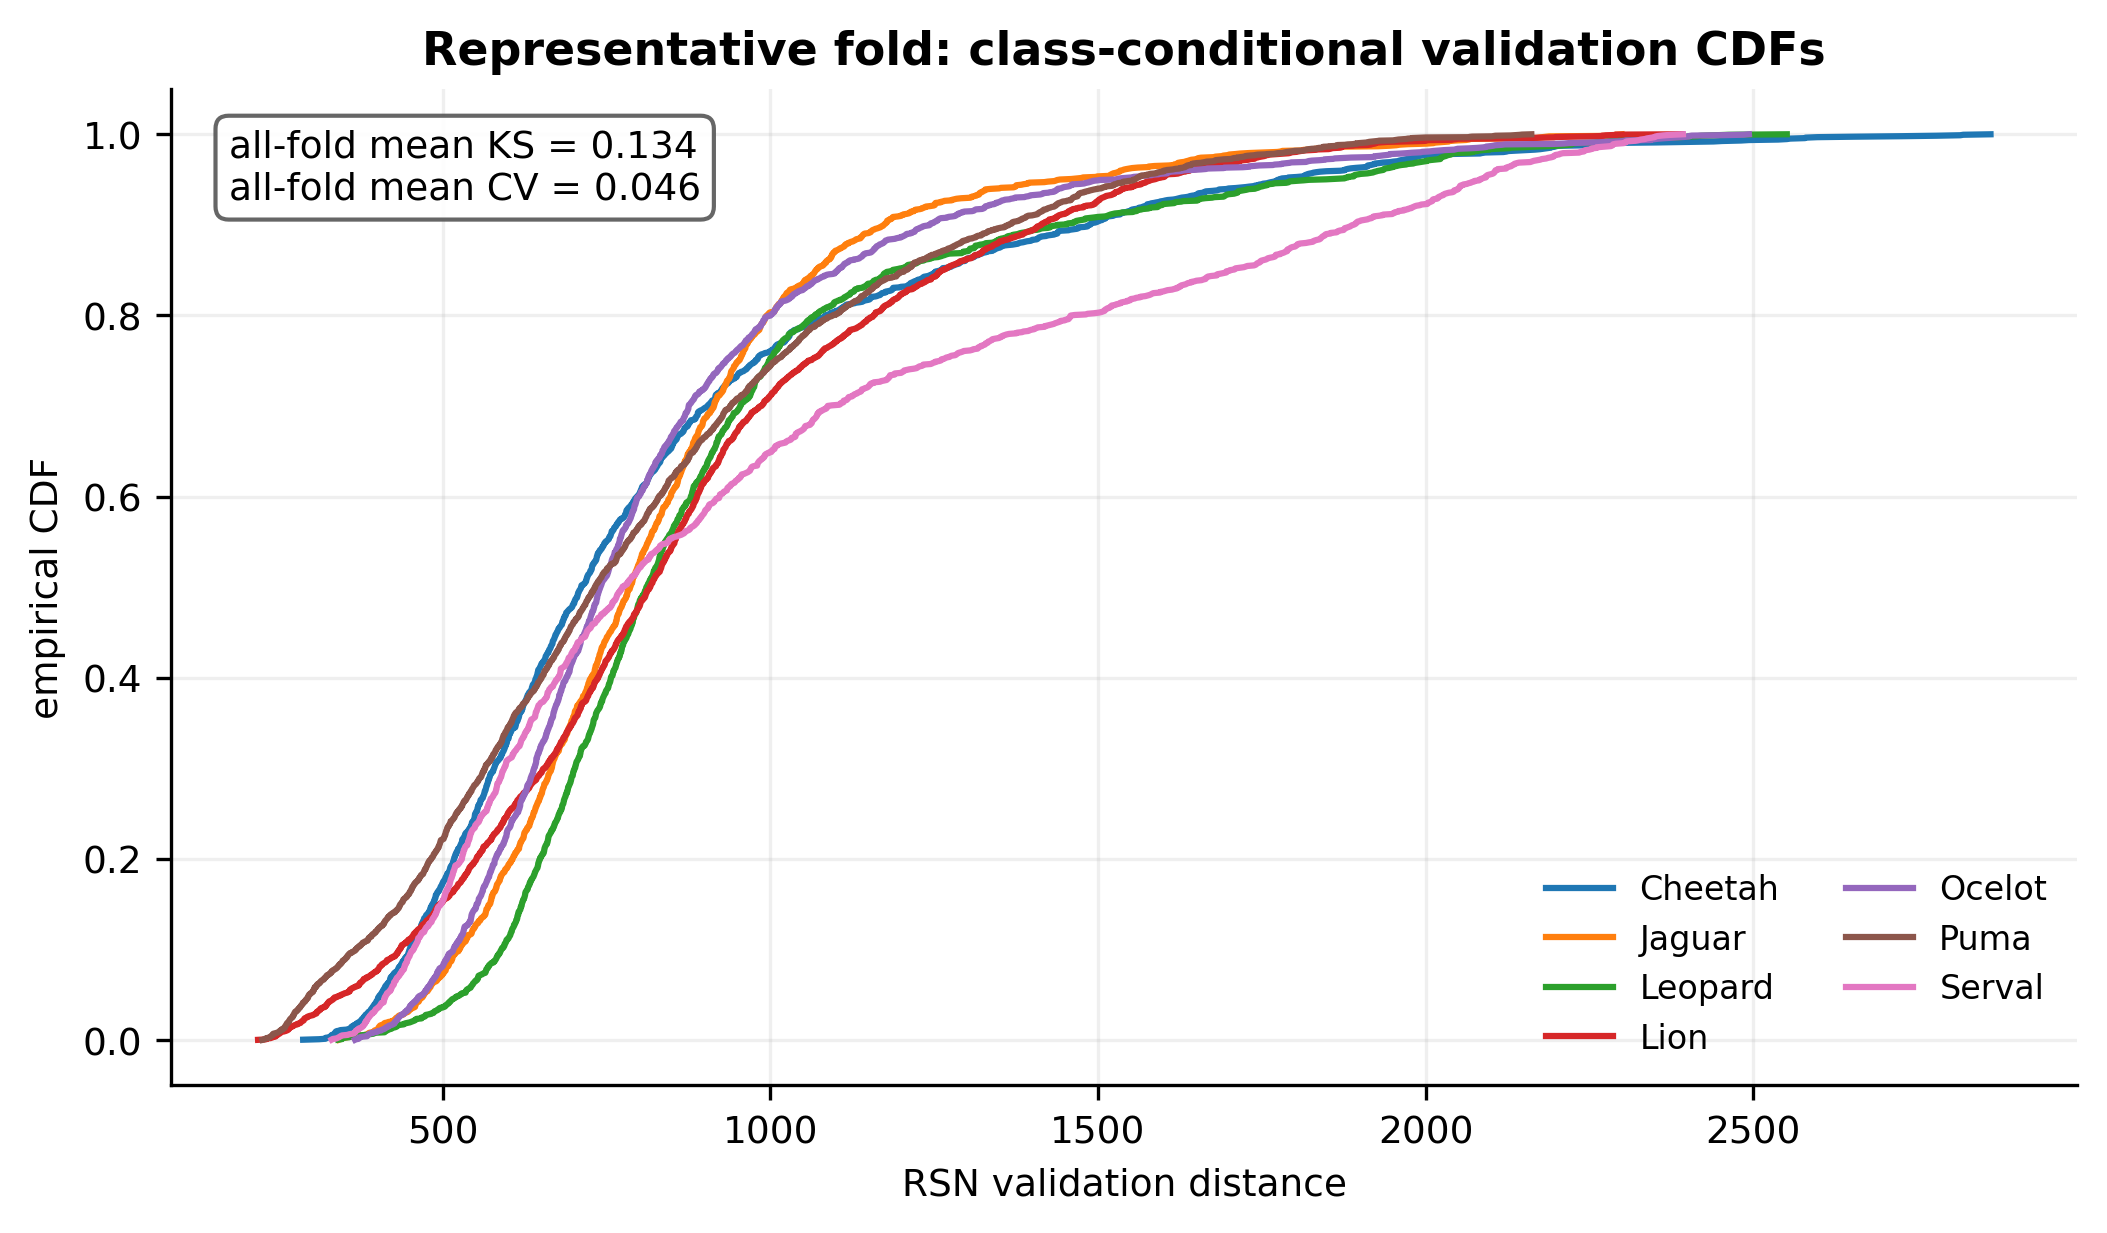
\includegraphics[width=\linewidth]{fig03_shared_shape_cdf.png}
  \caption{代表 fold のクラス別 validation 距離 CDF．数値は全1,476 foldの平均．}
  \label{fig:cdf}
\end{figure}

\subsection{Huber化と失敗モード}

Huber化は全体平均では小さいが安定した改善を与える．未知種別には差があり，全 $m$ 集計で cheetah は AUROC $+0.0011$，tiger と lion は約 $+0.0006$，leopard は $-0.0003$ であった．広い次元へ分散したOOD信号では単一座標ノイズの抑制が有効だが，少数次元に集中した信号では線形化が検出力も抑えうる．したがって Huber は主効果ではなく，対角標準化を安定化する補助要素と位置づけられる．

per-OOD-class結果は，距離標準化だけでは解けない限界も示す．tiger の AUROC 0.978に対し，jaguar，leopard，ocelot は0.840--0.847である．ロゼット模様を共有する種では，意味的には別種でも DINOv2 の局所支持が重なり，標準化後距離そのものが小さくなる．この場合，どの集約関数も失われた種識別情報を復元できない．改善には，部位対応，毛皮模様の局所表現，階層分類情報など，backbone側の表現を変える必要がある．

\subsection{生特徴・全クラス候補の含意}

DINOv2 特徴ノルムは画像品質，背景，対象の可視性などを含む可能性があり，$\ell_2$ 正規化は超近接種を分ける補助信号も除去しうる．また top-3候補制限は計算量を減らす一方，未知入力に対する ridge head の誤順位を scoreへ持ち込む．全クラス候補を用いる主設定は分類 headから独立し，問い合わせ当たりの主要計算量は通常の全bank \knn と同じ $O(ND)$，追加の Huber 集約は $O(CkD)$ である．ただし表~\ref{tab:ablation}の感度条件は正規化，$k$，候補数を同時に変えるため，各要因の因果的寄与を分離したものではない．

\section{限界}

本研究には次の限界がある．第一に，単一のネコ科8種とDINOv2特徴に限定しており，他分類群・他domain・他backboneへの外的妥当性は未確認である．第二に，ウェブ収集画像を自動・目視規則でクリーニングしたが，細かな誤ラベルや低品質画像が残る可能性がある．第三に，$m=7$ は48 foldと少なく，高 $m$ の手法差に対する区間は広い．第四に，同じ画像集合を異なるID/OOD組合せで再利用するため fold は完全独立ではなく，$t$近似の paired CI は設定間依存を過小評価しうる．第五に，特徴ノルムやロゼット種の解釈は観測結果と整合する仮説であり，局所部位介入などによる因果的検証ではない．

\section{結論}

超近接 OOD に対し，クラス条件付き次元別標準化と Huber 集約を用いる \RSN を提示した．クリーニング後105,554枚，$m=2$--7の全1,476 fold・21手法比較で，\RSN は \knn を全18条件で上回り，3指標すべての平均順位で首位となった．改善は特にFPR95で大きく，クラス固有の自然変動を境界付近で誤検出する問題への有効性を示す．一方，高 $m$ の AUROCでは OpenMax，AUPR-OUTでは RMD が強く，\RSN が全条件で最良ではないことも確認した．今後は分類群とbackboneを拡張し，ロゼット種のように局所支持が重なる失敗例へ部位・階層表現を導入する必要がある．

\appendix
\section{再現用設定}

主設定は \texttt{normalize=false, k=150, delta=1.345, min\_std=1e-3, candidate=all, calibrated=false} である．評価単位は \texttt{backbone, seed, id\_size, id\_set} の組であり，fold-level CSV は同じ単位で手法を paired に結合できる．検証済み実装は \texttt{src/maf07/methods/verified\_baselines.py}，全サイズ runner，完全性監査，集計はそれぞれ \texttt{scripts/run\_verified\_baseline\_sweep\_hades.sh}，\texttt{audit\_verified\_baseline\_sweep.py}，\texttt{aggregate\_verified\_baseline\_sweep.py} に保存した．完全なCSVは \texttt{docs/results/rsn\_baseline\_full\_20260711/} に置く．

{\footnotesize
\begin{thebibliography}{99}

\bibitem{hendrycks2017baseline}
D. Hendrycks and K. Gimpel,
``A Baseline for Detecting Misclassified and Out-of-Distribution Examples in Neural Networks,''
\textit{ICLR}, 2017.

\bibitem{norouzzadeh2018automatically}
M. S. Norouzzadeh et al.,
``Automatically identifying, counting, and describing wild animals in camera-trap images with deep learning,''
\textit{PNAS}, vol. 115, no. 25, 2018.

\bibitem{tuia2022perspectives}
D. Tuia et al.,
``Perspectives in machine learning for wildlife conservation,''
\textit{Nature Communications}, vol. 13, 2022.

\bibitem{sun2022knn}
Y. Sun, Y. Ming, X. Zhu, and Y. Li,
``Out-of-Distribution Detection with Deep Nearest Neighbors,''
\textit{ICML}, 2022.

\bibitem{liu2020energy}
W. Liu, X. Wang, J. Owens, and Y. Li,
``Energy-based Out-of-distribution Detection,''
\textit{NeurIPS}, 2020.

\bibitem{liu2023gen}
X. Liu, Y. Lochman, and C. Zach,
``GEN: Pushing the Limits of Softmax-Based Out-of-Distribution Detection,''
\textit{CVPR}, 2023.

\bibitem{huang2021gradnorm}
R. Huang, A. Geng, and Y. Li,
``On the Importance of Gradients for Detecting Distributional Shifts in the Wild,''
\textit{NeurIPS}, 2021.

\bibitem{bendale2016openmax}
A. Bendale and T. Boult,
``Towards Open Set Deep Networks,''
\textit{CVPR}, 2016.

\bibitem{lee2018simple}
K. Lee, K. Lee, H. Lee, and J. Shin,
``A Simple Unified Framework for Detecting Out-of-Distribution Samples and Adversarial Attacks,''
\textit{NeurIPS}, 2018.

\bibitem{ren2021simple}
J. Ren et al.,
``A Simple Fix to Mahalanobis Distance for Improving Near-OOD Detection,''
\textit{ICML Workshop}, 2021.

\bibitem{muller2025mahalanobispp}
M. M\"uller and M. Hein,
``Mahalanobis++: Improving OOD Detection via Feature Normalization,''
\textit{ICML}, 2025.

\bibitem{wang2022vim}
H. Wang, Z. Li, L. Feng, and W. Zhang,
``ViM: Out-of-Distribution with Virtual-Logit Matching,''
\textit{CVPR}, 2022.

\bibitem{oquab2024dinov2}
M. Oquab et al.,
``DINOv2: Learning Robust Visual Features without Supervision,''
\textit{TMLR}, 2024.

\bibitem{huber1964robust}
P. J. Huber,
``Robust Estimation of a Location Parameter,''
\textit{The Annals of Mathematical Statistics}, vol. 35, no. 1, 1964.

\bibitem{dkw1956}
A. Dvoretzky, J. Kiefer, and J. Wolfowitz,
``Asymptotic Minimax Character of the Sample Distribution Function and of the Classical Multinomial Estimator,''
\textit{The Annals of Mathematical Statistics}, vol. 27, no. 3, 1956.

\end{thebibliography}
}

\end{document}
